% Adjust these for the path of the theme and its graphics, relative to this file
%\usepackage{beamerthemeFalmouthGamesAcademy}
\usepackage{../../beamerthemeFalmouthGamesAcademy}
\usepackage{multimedia}
\graphicspath{ {../../} }

% Default language for code listings
\lstset{language=Python
}

% For strikethrough effect
\usepackage[normalem]{ulem}
\usepackage{wasysym}

\usepackage{algpseudocode}

\usepackage{pdfpages}

% http://www.texample.net/tikz/examples/state-machine/
\usetikzlibrary{arrows,automata}

\newcommand{\modulecode}{COMP260}\newcommand{\moduletitle}{Distributed Systems}\newcommand{\sessionnumber}{5}


\hypersetup{
pdftex,
pdftitle=\sessionnumber: Complexity,
pdfauthor=Ed Powley,
pdfdisplaydoctitle,
pdflang=en-GB
}
 
\begin{document}
\title{\sessionnumber: Complexity}
\subtitle{\modulecode: \moduletitle}

\frame{\titlepage} 

\newcommand{\namesunsorted}{
	\fbox{\parbox{0.9\textwidth}{\tiny
		Anderson, Martha \par
		Parker, Debra \par
		Russell, Mildred \par
		Stewart, Howard \par
		White, Amanda \par
		Perez, Diana \par
		Lewis, Rose \par
		Scott, Michelle \par
		Davis, Marilyn \par
		Cox, Shirley \par
		Young, Frank \par
		Collins, Jane \par
		Kelly, Philip \par
		Miller, Jeremy \par
		Clark, Stephanie \par
		Brown, Janet \par
		Diaz, Harold \par
		Hughes, Aaron \par
		Sanders, Phillip \par
		Williams, Billy \par
		Henderson, Lawrence \par
		Baker, Theresa \par
		Gonzalez, Adam \par
		Lopez, Jeffrey \par
		Ward, Jessica
	}}
}

\newcommand{\namessorted}{
	\fbox{\parbox{0.9\textwidth}{\tiny
		Anderson, Martha \par
		Baker, Theresa \par
		Brown, Janet \par
		Clark, Stephanie \par
		Collins, Jane \par
		Cox, Shirley \par
		Davis, Marilyn \par
		Diaz, Harold \par
		Gonzalez, Adam \par
		Henderson, Lawrence \par
		Hughes, Aaron \par
		Kelly, Philip \par
		Lewis, Rose \par
		Lopez, Jeffrey \par
		Miller, Jeremy \par
		Parker, Debra \par
		Perez, Diana \par
		Russell, Mildred \par
		Sanders, Phillip \par
		Scott, Michelle \par
		Stewart, Howard \par
		Ward, Jessica \par
		White, Amanda \par
		Williams, Billy \par
		Young, Frank
	}}
}

\begin{frame}{Search}
	\begin{columns}
		\begin{column}{0.3\textwidth}
			\namesunsorted
		\end{column}
		\begin{column}{0.66\textwidth}
			\begin{itemize}
				\item We have a list of names, each with some data associated \pause
				\item We want to find one of them
			\end{itemize}
		\end{column}
	\end{columns}
\end{frame}

\begin{frame}{Linear search}
	\begin{columns}
		\begin{column}{0.3\textwidth}
			\namesunsorted
		\end{column}
		\begin{column}{0.66\textwidth}
			\begin{algorithmic}
				\Procedure{Find}{name, list} \pause
					\For{each item in list} \pause
						\If{item.name $=$ name} \pause
							\State \textbf{return} item \pause
						\EndIf
					\EndFor
					\State \textbf{throw} ``Not found'' \pause
				\EndProcedure
			\end{algorithmic}
		\end{column}
	\end{columns}
\end{frame}

\begin{frame}{How long does it take?}
	Socrative room code: \texttt{FALCOMPED}
	\begin{itemize}
		\item Suppose there are 25 items in the list \pause
		\item In the \textbf{best case}, how many items do we need to visit before finding the one we want? \pause
		\item How about in the \textbf{worst case}?
	\end{itemize}
\end{frame}

\begin{frame}{How long does it take?}
	Socrative room code: \texttt{FALCOMPED}
	\begin{itemize}
		\item If there are 25 items in the list, the \textbf{worst case} number of items visited is 25 \pause
		\item How about if there are 50 items? \pause
		\item How about 100 items? \pause
		\item If the number of items \textbf{doubles}, what happens to the amount of time the search takes?
	\end{itemize}
\end{frame}

\begin{frame}{Linear time}
	\begin{columns}
		\begin{column}{0.45\textwidth}
			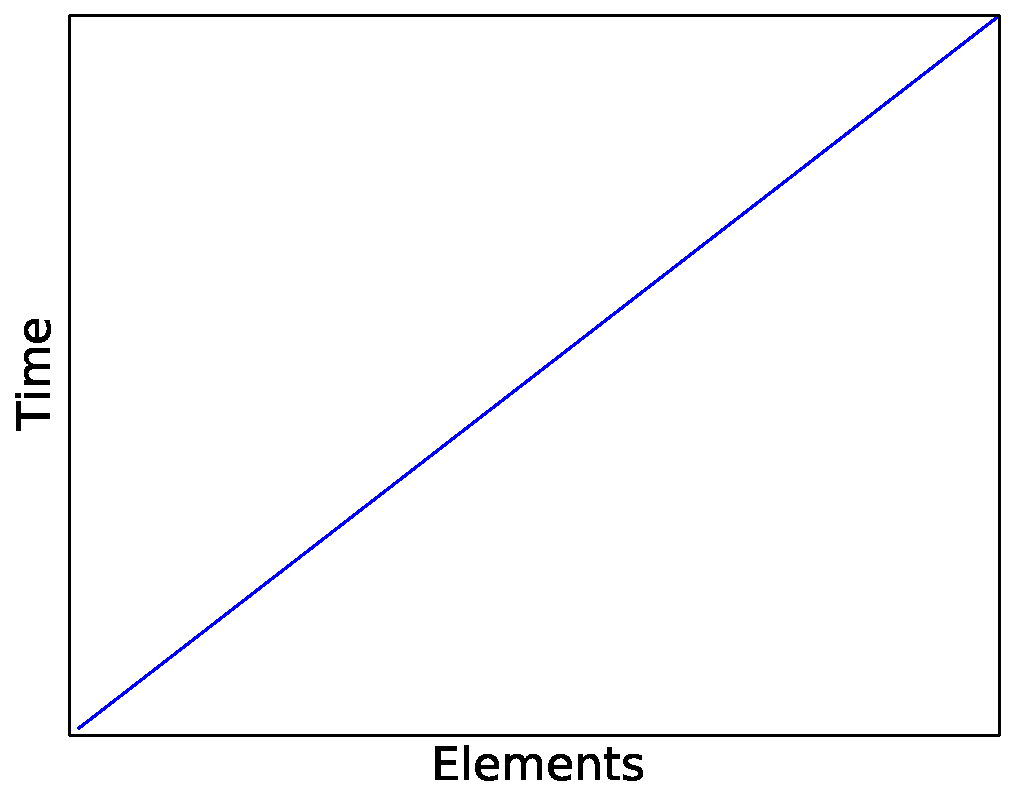
\includegraphics[width=\textwidth]{plot2_linear}
		\end{column}
		\begin{column}{0.55\textwidth}
			\begin{itemize}
				\item The running time of linear search is \textbf{proportional} to the size $n$ of the list \pause
				\item Linear search is said to have \textbf{linear time complexity} \pause
				\item Also written as \textbf{$O(n)$ time complexity}
			\end{itemize}
		\end{column}
	\end{columns}
\end{frame}

\begin{frame}{Searching a sorted list}
	\begin{columns}
		\begin{column}{0.3\textwidth}
			\namessorted
		\end{column}
		\begin{column}{0.66\textwidth}
			\begin{itemize}
				\item If the list is \textbf{sorted} in alphabetical order, we can do better than linear...
			\end{itemize}
		\end{column}
	\end{columns}
\end{frame}

\begin{frame}{Binary search}
	\begin{algorithmic}
		\Procedure{Find}{name, list} \pause
			\If{list is empty}
				\State \textbf{throw} ``Not found''
			\EndIf \pause
			\State mid $\gets$ the ``middle'' item of the list \pause
			\If{name $=$ mid.name}
				\State \textbf{return} mid \pause
			\ElsIf{name $<$ mid.name}
				\State \textbf{return} \Call{Find}{name, first half of list} \pause
			\ElsIf{name $>$ mid.name}
				\State \textbf{return} \Call{Find}{name, second half of list} \pause
			\EndIf
		\EndProcedure
	\end{algorithmic}
\end{frame}

\begin{frame}{Find ``Lopez, Jeffrey''}
	\begin{columns}
		\begin{column}{0.3\textwidth}
			\fbox{\parbox{0.9\textwidth}{\tiny
				$\phantom\longrightarrow$ Anderson, Martha \par
				$\phantom\longrightarrow$ Baker, Theresa \par
				$\phantom\longrightarrow$ Brown, Janet \par
				$\phantom\longrightarrow$ Clark, Stephanie \par
				$\phantom\longrightarrow$ Collins, Jane \par
				$\phantom\longrightarrow$ Cox, Shirley \par
				$\phantom\longrightarrow$ Davis, Marilyn \par
				$\phantom\longrightarrow$ Diaz, Harold \par
				$\phantom\longrightarrow$ Gonzalez, Adam \par
				$\phantom\longrightarrow$ Henderson, Lawrence \par
				$\phantom\longrightarrow$ Hughes, Aaron \par
				$\phantom\longrightarrow$ Kelly, Philip \par
				$\longrightarrow$ Lewis, Rose \par
				$\phantom\longrightarrow$ Lopez, Jeffrey \par
				$\phantom\longrightarrow$ Miller, Jeremy \par
				$\phantom\longrightarrow$ Parker, Debra \par
				$\phantom\longrightarrow$ Perez, Diana \par
				$\phantom\longrightarrow$ Russell, Mildred \par
				$\phantom\longrightarrow$ Sanders, Phillip \par
				$\phantom\longrightarrow$ Scott, Michelle \par
				$\phantom\longrightarrow$ Stewart, Howard \par
				$\phantom\longrightarrow$ Ward, Jessica \par
				$\phantom\longrightarrow$ White, Amanda \par
				$\phantom\longrightarrow$ Williams, Billy \par
				$\phantom\longrightarrow$ Young, Frank
			}}
		\end{column}
	\end{columns}
\end{frame}

\begin{frame}{Find ``Lopez, Jeffrey''}
	\begin{columns}
		\begin{column}{0.3\textwidth}
			\fbox{\parbox{0.9\textwidth}{\tiny
				{\color{gray}
				$\phantom\longrightarrow$ Anderson, Martha \par
				$\phantom\longrightarrow$ Baker, Theresa \par
				$\phantom\longrightarrow$ Brown, Janet \par
				$\phantom\longrightarrow$ Clark, Stephanie \par
				$\phantom\longrightarrow$ Collins, Jane \par
				$\phantom\longrightarrow$ Cox, Shirley \par
				$\phantom\longrightarrow$ Davis, Marilyn \par
				$\phantom\longrightarrow$ Diaz, Harold \par
				$\phantom\longrightarrow$ Gonzalez, Adam \par
				$\phantom\longrightarrow$ Henderson, Lawrence \par
				$\phantom\longrightarrow$ Hughes, Aaron \par
				$\phantom\longrightarrow$ Kelly, Philip \par
				$\phantom\longrightarrow$ Lewis, Rose \par
				}
				$\phantom\longrightarrow$ Lopez, Jeffrey \par
				$\phantom\longrightarrow$ Miller, Jeremy \par
				$\phantom\longrightarrow$ Parker, Debra \par
				$\phantom\longrightarrow$ Perez, Diana \par
				$\phantom\longrightarrow$ Russell, Mildred \par
				$\longrightarrow$ Sanders, Phillip \par
				$\phantom\longrightarrow$ Scott, Michelle \par
				$\phantom\longrightarrow$ Stewart, Howard \par
				$\phantom\longrightarrow$ Ward, Jessica \par
				$\phantom\longrightarrow$ White, Amanda \par
				$\phantom\longrightarrow$ Williams, Billy \par
				$\phantom\longrightarrow$ Young, Frank
			}}
		\end{column}
	\end{columns}
\end{frame}

\begin{frame}{Find ``Lopez, Jeffrey''}
	\begin{columns}
		\begin{column}{0.3\textwidth}
			\fbox{\parbox{0.9\textwidth}{\tiny
				{\color{gray}
				$\phantom\longrightarrow$ Anderson, Martha \par
				$\phantom\longrightarrow$ Baker, Theresa \par
				$\phantom\longrightarrow$ Brown, Janet \par
				$\phantom\longrightarrow$ Clark, Stephanie \par
				$\phantom\longrightarrow$ Collins, Jane \par
				$\phantom\longrightarrow$ Cox, Shirley \par
				$\phantom\longrightarrow$ Davis, Marilyn \par
				$\phantom\longrightarrow$ Diaz, Harold \par
				$\phantom\longrightarrow$ Gonzalez, Adam \par
				$\phantom\longrightarrow$ Henderson, Lawrence \par
				$\phantom\longrightarrow$ Hughes, Aaron \par
				$\phantom\longrightarrow$ Kelly, Philip \par
				$\phantom\longrightarrow$ Lewis, Rose \par
				}
				$\phantom\longrightarrow$ Lopez, Jeffrey \par
				$\phantom\longrightarrow$ Miller, Jeremy \par
				$\longrightarrow$ Parker, Debra \par
				$\phantom\longrightarrow$ Perez, Diana \par
				$\phantom\longrightarrow$ Russell, Mildred \par
				{\color{gray}$\phantom\longrightarrow$ Sanders, Phillip \par
				$\phantom\longrightarrow$ Scott, Michelle \par
				$\phantom\longrightarrow$ Stewart, Howard \par
				$\phantom\longrightarrow$ Ward, Jessica \par
				$\phantom\longrightarrow$ White, Amanda \par
				$\phantom\longrightarrow$ Williams, Billy \par
				$\phantom\longrightarrow$ Young, Frank
				}
			}}
		\end{column}
	\end{columns}
\end{frame}

\begin{frame}{Find ``Lopez, Jeffrey''}
	\begin{columns}
		\begin{column}{0.3\textwidth}
			\fbox{\parbox{0.9\textwidth}{\tiny
				{\color{gray}
				$\phantom\longrightarrow$ Anderson, Martha \par
				$\phantom\longrightarrow$ Baker, Theresa \par
				$\phantom\longrightarrow$ Brown, Janet \par
				$\phantom\longrightarrow$ Clark, Stephanie \par
				$\phantom\longrightarrow$ Collins, Jane \par
				$\phantom\longrightarrow$ Cox, Shirley \par
				$\phantom\longrightarrow$ Davis, Marilyn \par
				$\phantom\longrightarrow$ Diaz, Harold \par
				$\phantom\longrightarrow$ Gonzalez, Adam \par
				$\phantom\longrightarrow$ Henderson, Lawrence \par
				$\phantom\longrightarrow$ Hughes, Aaron \par
				$\phantom\longrightarrow$ Kelly, Philip \par
				$\phantom\longrightarrow$ Lewis, Rose \par
				}
				$\longrightarrow$ Lopez, Jeffrey \par
				$\phantom\longrightarrow$ Miller, Jeremy \par
				{\color{gray}$\phantom\longrightarrow$ Parker, Debra \par
				$\phantom\longrightarrow$ Perez, Diana \par
				$\phantom\longrightarrow$ Russell, Mildred \par
				$\phantom\longrightarrow$ Sanders, Phillip \par
				$\phantom\longrightarrow$ Scott, Michelle \par
				$\phantom\longrightarrow$ Stewart, Howard \par
				$\phantom\longrightarrow$ Ward, Jessica \par
				$\phantom\longrightarrow$ White, Amanda \par
				$\phantom\longrightarrow$ Williams, Billy \par
				$\phantom\longrightarrow$ Young, Frank
				}
			}}
		\end{column}
	\end{columns}
\end{frame}

\begin{frame}{How long does it take?}
	Socrative room code: \texttt{FALCOMPED}
	\begin{columns}
		\begin{column}{0.55\textwidth}
			\begin{itemize}
				\item Each iteration cuts the list in \textbf{half} \pause
				\item Worst case: we have to keep halving until we get down to a single element \pause
				\item If the size of the list is \textbf{doubled}, what happens to the worst-case
					\textbf{number of iterations} required? \pause
				\item \textbf{Answer:} it increases by 1 \pause
				\item The running time is \textbf{logarithmic} or $O(\log n)$ \pause
			\end{itemize}
		\end{column}
		\begin{column}{0.45\textwidth}
			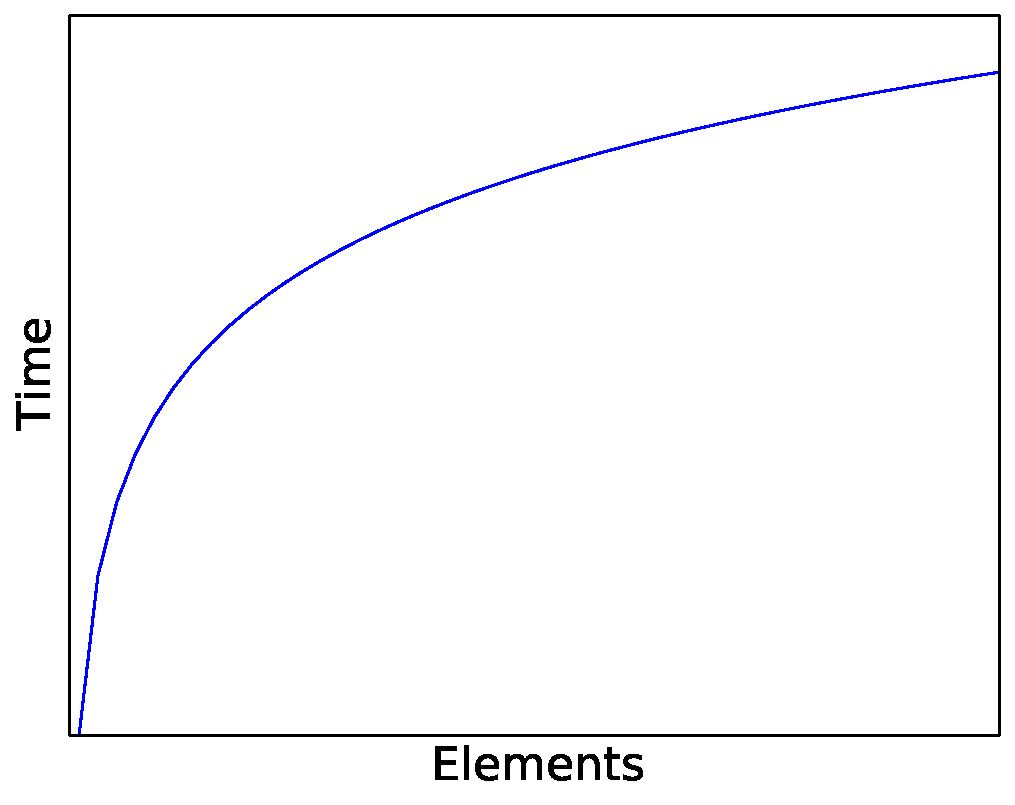
\includegraphics[width=\textwidth]{plot2_log}
		\end{column}
	\end{columns}
\end{frame}

\begin{frame}{Hidden complexity}
	\begin{algorithmic}
			\If{name $<$ mid.name}
				\State \textbf{return} \Call{Find}{name, first half of list}
			\ElsIf{name $>$ mid.name}
				\State \textbf{return} \Call{Find}{name, second half of list}
			\EndIf
	\end{algorithmic}
	\pause
	\begin{columns}
		\begin{column}{0.45\textwidth}
			\only<4->{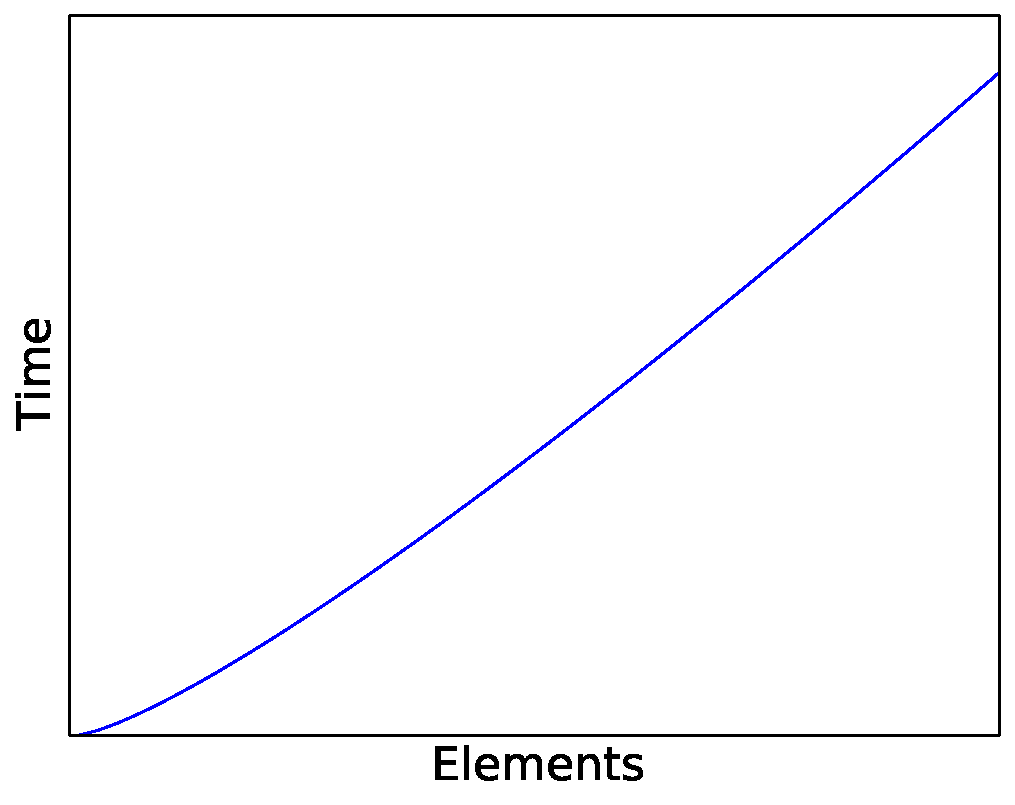
\includegraphics[width=\textwidth]{plot2_nlogn}}
		\end{column}
		\begin{column}{0.55\textwidth}
			\begin{itemize}
				\item Careful how you implement this! \pause
				\item \textbf{Copying} (half of) a list is \textbf{linear} $O(n)$ \pause
				\item The actual running time would be $O(n \log n)$ \pause
				\item Use \textbf{pointers} into the list instead of copying
			\end{itemize}
		\end{column}
	\end{columns}
\end{frame}

\begin{frame}{Binary search done wrong}
	\lstinputlisting{binary_search_bad.py}
\end{frame}

\begin{frame}{Binary search done right}
	\lstinputlisting{binary_search_good.py}
\end{frame}

\begin{frame}{Binary search vs linear search}
	Socrative room code: \texttt{FALCOMPED}
	\begin{columns}
		\begin{column}{0.45\textwidth}
			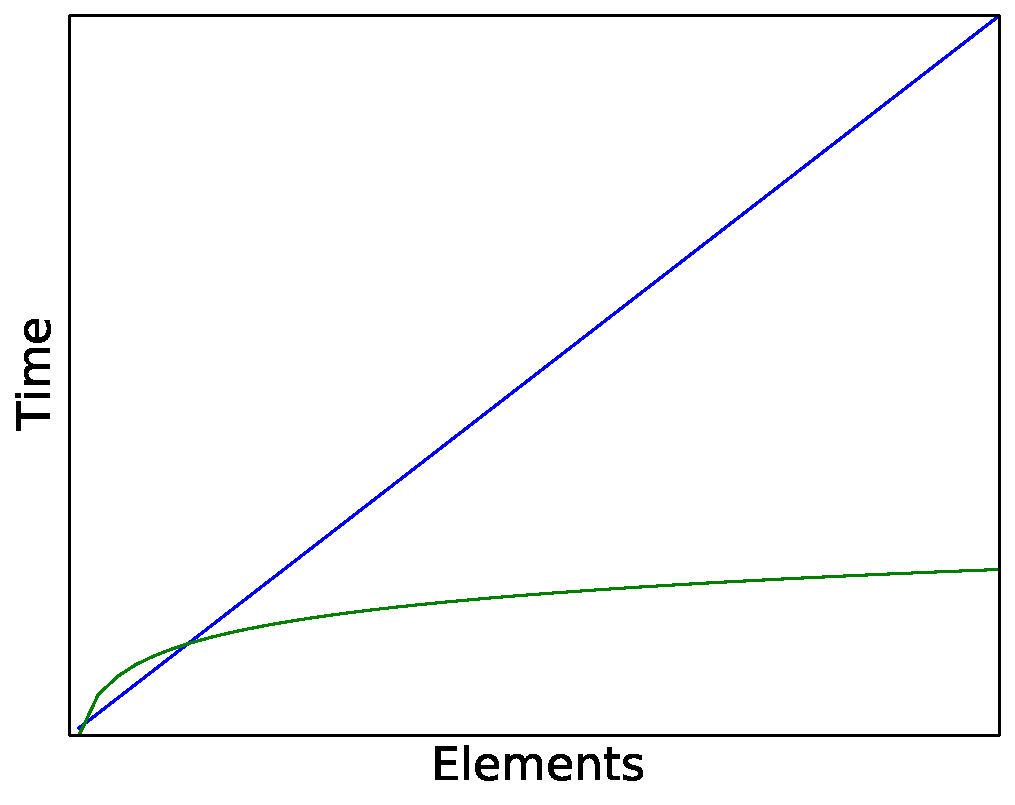
\includegraphics[width=\textwidth]{plot2_linear_log}
		\end{column}
		\begin{column}{0.55\textwidth}
			\begin{itemize}
				\item So binary search is better than linear search... right? \pause
				\item Discuss in \textbf{pairs}
				\item On Socrative, post \textbf{one reason} why, or \textbf{one situation} where,
					linear search may be a better choice than binary search
			\end{itemize}
		\end{column}
	\end{columns}
\end{frame}

\iffalse
\begin{frame}{Hashing}
	\begin{columns}
		\begin{column}{0.66\textwidth}
			\begin{itemize}
				\item Come up with a \textbf{hashing function} which maps elements to numbers \pause
				\item Example: assign $A=1, B=2, C=3$ etc, and add them together \pause
				\item Use these numbers to assign each element to a ``bin'' where it can be found \pause
			\end{itemize}
		\end{column}
		\begin{column}{0.3\textwidth}
			{\tiny
			\begin{tabular}{|c|l|}
$\vdots$ & $\vdots$ \\\hline
112 & Ward, Jessica \\\hline
113 & Baker, Theresa \\\hline
114 & Collins, Jane \\\hline
115 & --- \\\hline
116 & --- \\\hline
117 & Hughes, Aaron \\\hline
118 & --- \\\hline
119 & --- \\\hline
120 & --- \\\hline
121 & --- \\\hline
122 & Brown, Janet \\\hline
123 & --- \\\hline
124 & --- \\\hline
125 & Gonzalez, Adam \\ & Lewis, Rose \\\hline
126 & --- \\\hline
127 & --- \\\hline
128 & --- \\\hline
129 & --- \\\hline
130 & --- \\\hline
131 & --- \\\hline
132 & Young, Frank \\\hline
$\vdots$ & $\vdots$
			\end{tabular}
			}
		\end{column}
	\end{columns}
\end{frame}

\begin{frame}{Hash look-up}
	\begin{columns}
		\begin{column}{0.3\textwidth}
			{\tiny
			\begin{tabular}{|c|l|} \hline
				98 & Diaz, Harold \\\hline99 & Parker, Debra \\ & Perez, Diana \\ & White, Amanda \\\hline112 & Ward, Jessica \\\hline113 & Baker, Theresa \\\hline114 & Collins, Jane \\\hline117 & Hughes, Aaron \\\hline122 & Brown, Janet \\\hline125 & Gonzalez, Adam \\ & Lewis, Rose \\\hline132 & Young, Frank \\\hline135 & Kelly, Philip \\\hline138 & Cox, Shirley \\\hline142 & Clark, Stephanie \\\hline144 & Scott, Michelle \\\hline145 & Miller, Jeremy \\\hline147 & Davis, Marilyn \\\hline149 & Lopez, Jeffrey \\\hline151 & Anderson, Martha \\\hline158 & Williams, Billy \\\hline162 & Sanders, Phillip \\\hline171 & Russell, Mildred \\\hline175 & Stewart, Howard \\\hline183 & Henderson, Lawrence \\\hline
			\end{tabular}
			}
		\end{column}
		\begin{column}{0.66\textwidth}
			``Lopez, Jeffrey'' \pause
			
			$12 + 15 + 16 + 5 + 26 + 10 + 5 + 6 + 6 + 18 + 5 + 25 = 149$
		\end{column}
	\end{columns}
\end{frame}

\begin{frame}{How long does it take?}
	\begin{columns}
		\begin{column}{0.45\textwidth}
			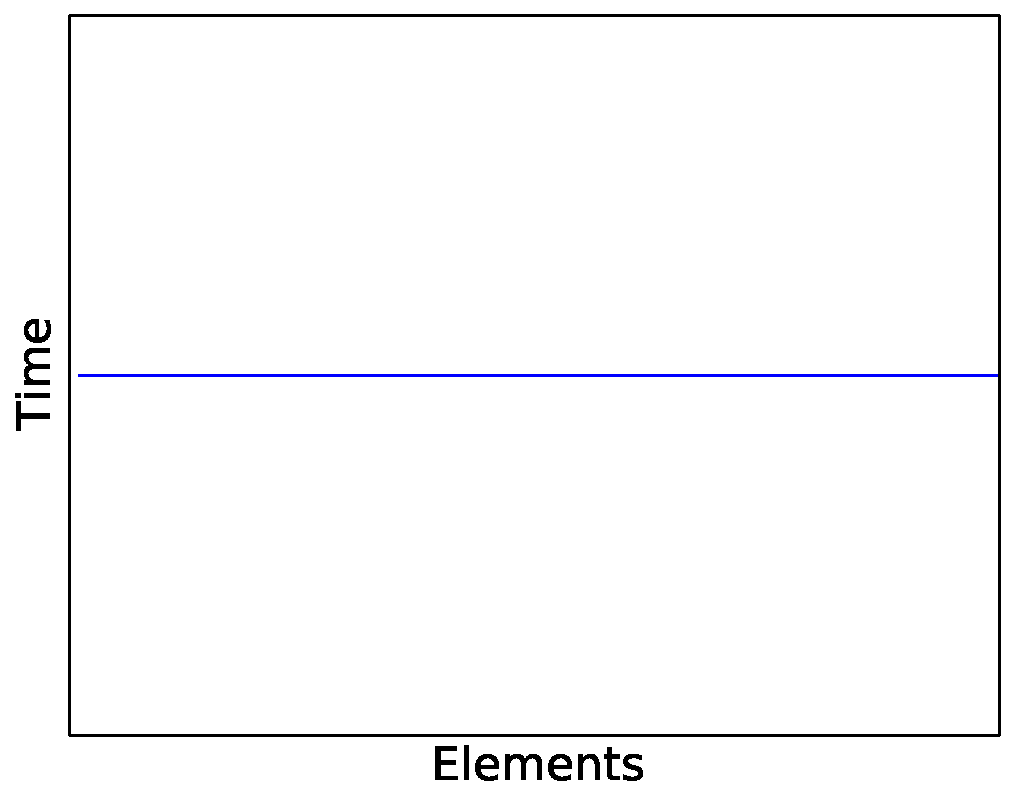
\includegraphics[width=\textwidth]{plot2_constant}
		\end{column}
		\begin{column}{0.55\textwidth}
			\begin{itemize}
				\item If there are no ``collisions'', look-up time is \textbf{constant} or $O(1)$ \pause
					\begin{itemize}
						\item (NB: constant \textbf{with respect to} $n$) \pause
					\end{itemize}
				\item I.e. doubling the size of the list \textbf{does not change} the look-up time \pause
				\item When there are collisions, need to fall back on something like linear or binary search within each bin
			\end{itemize}
		\end{column}
	\end{columns}
\end{frame}
\fi

\begin{frame}{More complexity classes}
	\begin{center}
		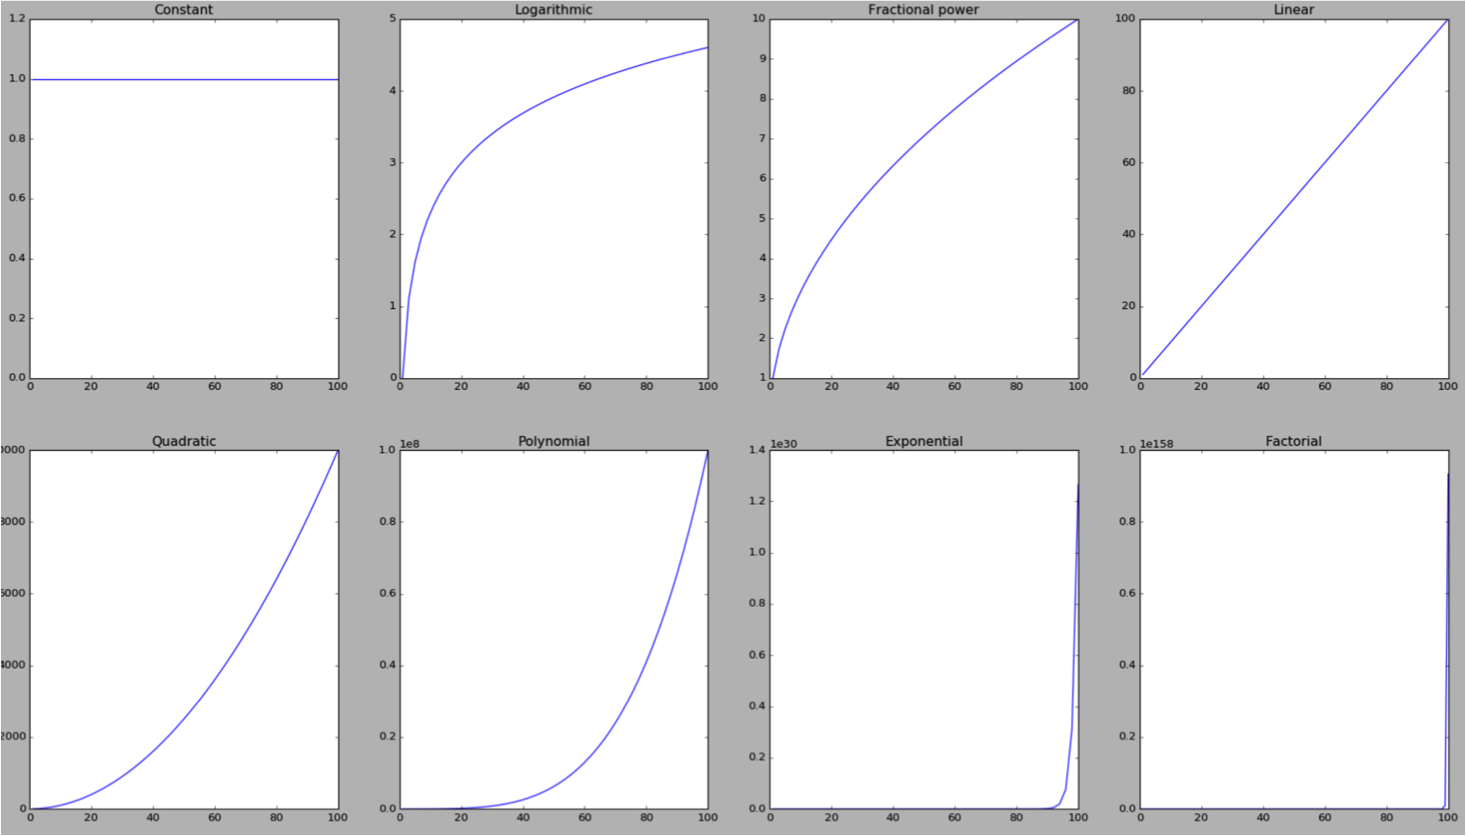
\includegraphics[width=\textwidth]{complexity_classes}
	\end{center}
\end{frame}

\begin{frame}{Complexity in games}
	\begin{columns}
		\begin{column}{0.4\textwidth}
			\only<3->{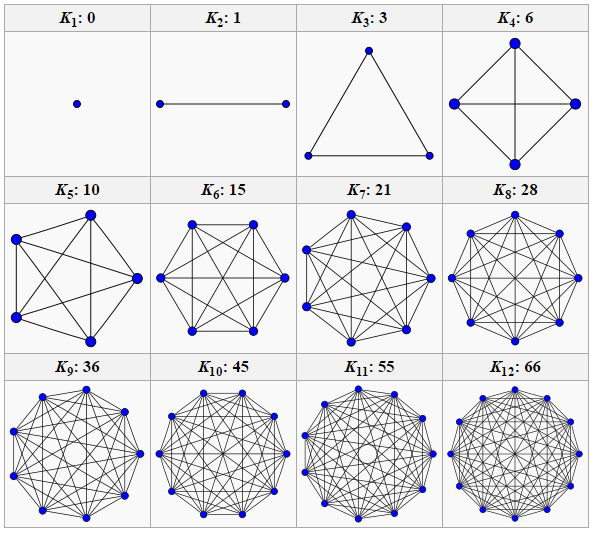
\includegraphics[width=\textwidth]{complete_graph}}
		\end{column}
		\begin{column}{0.6\textwidth}
			\begin{itemize}
				\item Example: collision detection between $n$ objects \pause
				\item The na\"ive way: check \textbf{each pair} of objects to see whether they have collided \pause
				\item This is \textbf{quadratic} or $O(n^2)$ \pause
				\item Doubling the number of objects would \textbf{quadruple} the time required! \pause
				\item Cleverer methods exist that are more scalable \pause
					\begin{itemize}
						\item Further reading: spatial hashing, quadtrees, octrees, Verlet lists
					\end{itemize}
			\end{itemize}
		\end{column}
	\end{columns}
\end{frame}

\begin{frame}{Caveats}
	\begin{itemize}
		\item We've used search as an example, but don't reinvent the wheel! \pause
			\begin{itemize}
				\item Most languages have existing implementations of linear and binary search on arrays or lists \pause
				\item Most languages have a \textbf{dictionary} data structure based on \textbf{hashing},
					which is generally better for this kind of key $\to$ value look-up
			\end{itemize}
	\end{itemize}
\end{frame}

\begin{frame}{Caveats}
	\begin{itemize}
		\item Time complexity only tells us how an algorithm \textbf{scales} with the size of the input \pause
			\begin{itemize}
				\item If we know the input will always be \textbf{small}, time complexity is not so important \pause
				\item Linear search is quicker than binary search if you only ever have 3 elements \pause
				\item Na\"ive collision detection is fine if your game only ever has 4 objects on screen \pause
				\item Sometimes complexity in terms of other resources (e.g.\ space, bandwidth) are more important than time \pause
			\end{itemize}
		\item Software development is all about choosing \textbf{the right tool for the job} \pause
			\begin{itemize}
				\item If you need scalability, choose a scalable algorithm \pause
				\item Otherwise, choose simplicity
			\end{itemize}
	\end{itemize}
\end{frame}

\begin{frame}{Summary}
	\begin{itemize}
		\item Time complexity tells us how the running time of an algorithm \textbf{scales} with the size of the data
			it is given \pause
		\item Choice of data structures and algorithms can have a large impact on the efficiency of your software \pause
		\item ... but only if scalability is actually a factor
	\end{itemize}
\end{frame}


\part{More on complexity}
\frame{\partpage}

\begin{frame}{Common complexity classes}
	\begin{center}
		\begin{tabular}{clc}
			\pause ``Faster'' & Constant & $O(1)$ \\
			\pause $\uparrow$ & Logarithmic & $O(\log n)$ \\
			\pause $|$ & Fractional power & $O(n^k)$, $k < 1$ \\
			\pause $|$ & Linear & $O(n)$ \\
			\pause $|$ & Quadratic & $O(n^2)$ \\
			\pause $|$ & Polynomial & $O(n^k)$, $k > 1$  \\
			\pause $\downarrow$ & Exponential & $O(e^n)$ \\
			\pause ``Slower'' & Factorial & $O(n!)$
		\end{tabular}
	\end{center}
\end{frame}

\begin{frame}{Common complexity classes}
	\begin{center}
		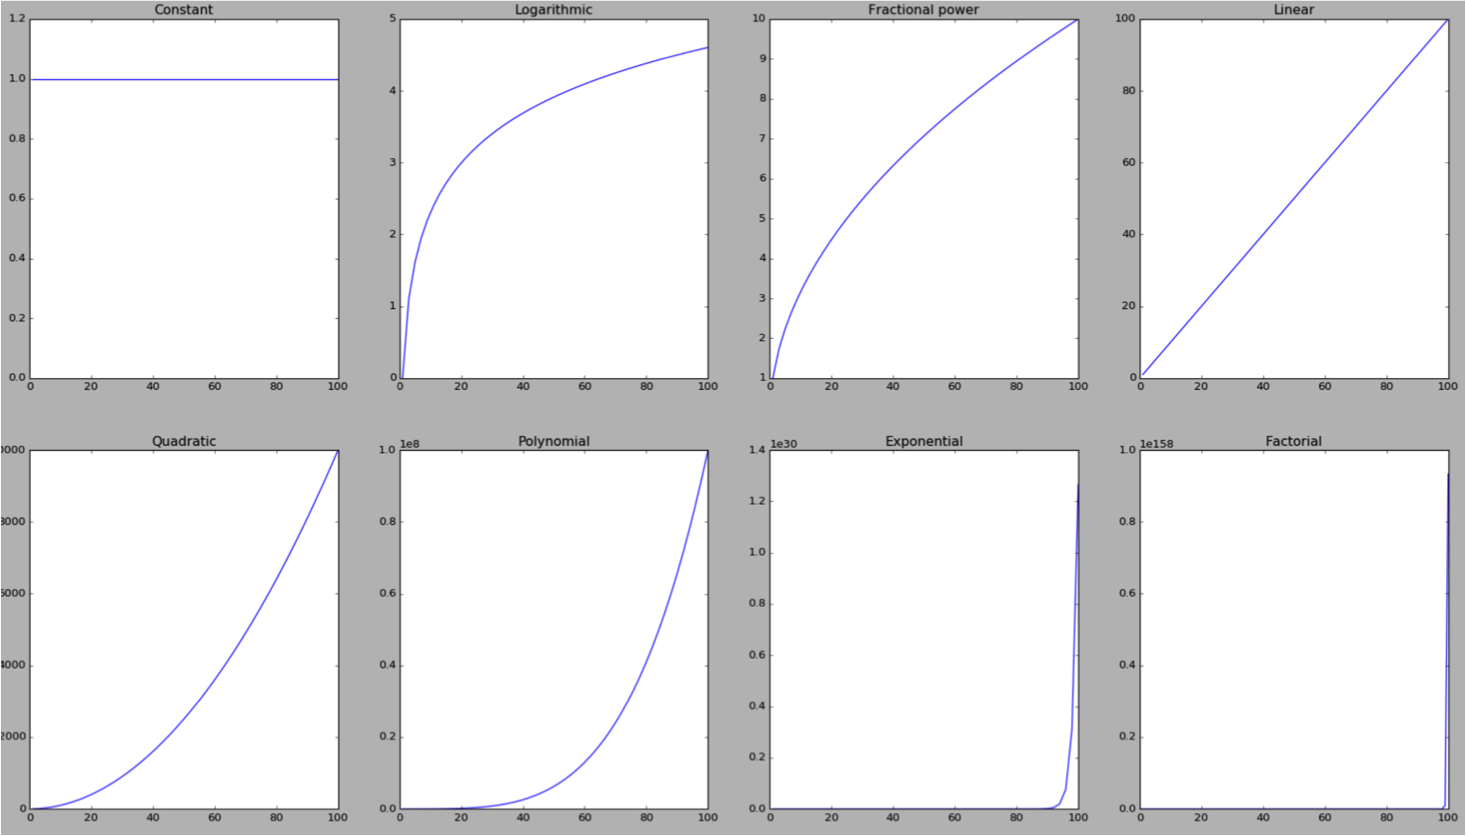
\includegraphics[width=\textwidth]{complexity_classes}
	\end{center}
\end{frame}

\begin{frame}{Working with big $O$ notation}
	\begin{itemize}
		\pause\item Can ignore \textbf{leading constants}
			\begin{itemize}
				\pause\item If one algorithm takes $n^2$ operations,
					another takes $500n^2$
					and a third takes $0.00000001n^2$,
					all three are $O(n^2)$
			\end{itemize}
		\pause\item Take only the \textbf{dominant term}
			\begin{itemize}
				\pause\item The term that is largest when $n$ is large
				\pause\item If an algorithm takes $0.1n^3 + 300n^2 + 7000$ operations,
					it is $O(n^3)$
			\end{itemize}
		\pause\item Multiply \textbf{compound} algorithms
			\begin{itemize}
				\pause\item If an algorithm does $n$ ``things'' and each ``thing'' is $O(n)$,
					then the overall algorithm is $O(n^2)$
			\end{itemize}
	\end{itemize}
\end{frame}

\begin{frame}{Quadratic complexity}
	\begin{columns}
		\begin{column}{0.4\textwidth}
			\only<3->{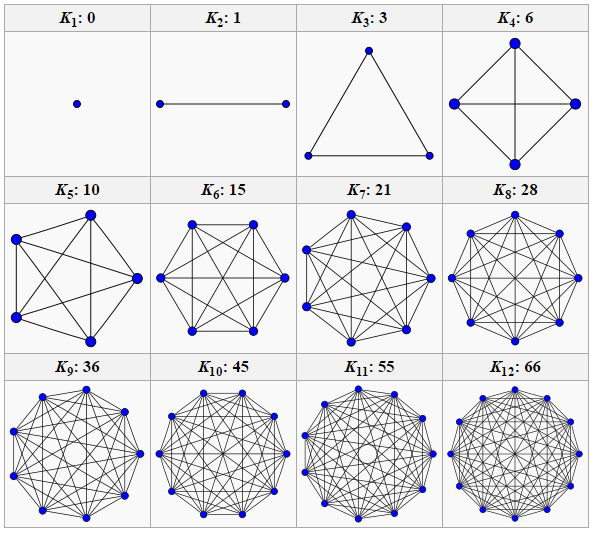
\includegraphics[width=\textwidth]{complete_graph}}
		\end{column}
		\begin{column}{0.6\textwidth}
			\begin{itemize}
				\item Collision detection between $n$ objects \pause
				\item The na\"ive way: check \textbf{each pair} of objects to see whether they have collided \pause
				\item This is \textbf{quadratic} or $O(n^2)$ \pause
				\item Doubling the number of objects would \textbf{quadruple} the time required! \pause
				\item Cleverer methods exist that are more scalable \pause
					\begin{itemize}
						\item Further reading: spatial hashing, quadtrees, octrees, Verlet lists
					\end{itemize}
			\end{itemize}
		\end{column}
	\end{columns}
\end{frame}

\begin{frame}{Exponential complexity}
	\begin{itemize}
		\pause\item A \text{prime number} is a number that is divisible only by $1$ and itself
		\pause\item Given an $n$-bit number $m = pq$ that is a product of two primes $p$ and $q$, find $p$ and $q$.
	\end{itemize}
	\pause
	\begin{algorithmic}
		\For{$p = 2, 3, \dots, m$}
			\State $q \gets m / p$
			\If{$q$ is an integer}
				\State \textbf{return} $p,q$
			\EndIf
		\EndFor
	\end{algorithmic}
	\begin{itemize}
		\pause\item Since $m \leq 2^n-1$, in the worst case this is $O(2^n)$
			\begin{itemize}
				\pause\item Actually even slower because division is not $O(1)$
			\end{itemize}
		\pause\item Adding 1 to $n$ potentially \textbf{doubles} the running time!
	\end{itemize}
\end{frame}

\begin{frame}{Exponential complexity}
	\begin{itemize}
		\pause\item If adding 1 bit \textbf{doubles} the running time...
		\pause\item Suppose factoring a 16-bit number takes 1 millisecond
		\pause\item Factoring a 32-bit number would take 65.5 seconds
		\pause\item Factoring a 48-bit number would take 49.7 days
		\pause\item Factoring a 64-bit number would take 8919 years
		\pause\item Factoring a 96-bit number would take 2800 times the age of the universe
	\end{itemize}
\end{frame}

\begin{frame}{Aside: a famous unanswered question in computing}
	\begin{itemize}
		\pause\item A problem is ``in $P$'' if it can be solved with an
			algorithm running in $O(n^k)$ time
		\pause\item A problem is in $NP$ if a potential solution can be checked in $O(n^k)$ time
			\begin{itemize}
				\pause\item Equivalently, it can be solved with an algorithm running in $O(n^k)$ time on an infinitely parallel machine
			\end{itemize}
		\pause\item Are there any problems in $NP$ but not in $P$?
	\end{itemize}
\end{frame}

\begin{frame}{P versus NP}
	\begin{itemize}
		\pause\item If you can find a \textbf{mathematical proof} that either $P = NP$ or $P \neq NP$, there's a \$1 million prize...
		\pause\item It is believed that $P \neq NP$, so large instances of
			$NP$-hard problems are not solvable in a feasible amount of time
			\begin{itemize}
				\pause\item Many types of cryptography are based on this assumption
				\pause\item Quantum computers are ``infinitely parallel'' in a sense
					so \emph{can} solve some large $NP$-hard problems
			\end{itemize}
	\end{itemize}
\end{frame}

\begin{frame}{Caveats}
	\begin{itemize}
		\item Time complexity only tells us how an algorithm \textbf{scales} with the size of the input \pause
			\begin{itemize}
				\item If we know the input will always be \textbf{small}, time complexity is not so important \pause
				\item Linear search is quicker than binary search if you only ever have 3 elements \pause
				\item Na\"ive collision detection is fine if your game only ever has 4 objects on screen \pause
				\item Sometimes complexity in terms of other resources (e.g.\ space, bandwidth) are more important than time \pause
			\end{itemize}
		\item Software development is all about choosing \textbf{the right tool for the job} \pause
			\begin{itemize}
				\item If you need scalability, choose a scalable algorithm \pause
				\item Otherwise, choose simplicity
			\end{itemize}
	\end{itemize}
\end{frame}

\begin{frame}{Summary}
	\begin{itemize}
		\item Time complexity tells us how the running time of an algorithm \textbf{scales} with the size of the data
			it is given \pause
		\item Choice of data structures and algorithms can have a large impact on the efficiency of your software \pause
		\item ... but only if scalability is actually a factor
	\end{itemize}
\end{frame}


\part{Turing machines}
\frame{\partpage}

\begin{frame}{Turing machines}
    \begin{center}
        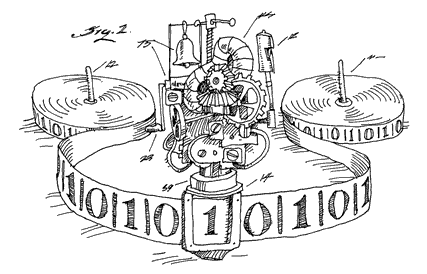
\includegraphics[width=0.6\textwidth]{turing_machine}
        % Image from https://medium.com/@calhoun137/alan-turings-universal-computing-machine-be69c052c6fd
    \end{center}
    \begin{itemize}
        \pause\item Introduced in 1936 by Alan Turing
        \pause\item Theoretical model of a ``computer''
            \begin{itemize}
                \pause\item I.e.\ a machine that carries out computations (calculations)
            \end{itemize}
    \end{itemize}
\end{frame}

\begin{frame}{Turing machine}
    \begin{itemize}
        \pause\item Has a finite number of \textbf{states}
        \pause\item Has an infinite \textbf{tape}
        \pause\item Each space on the tape holds a \textbf{symbol} from a finite \textbf{alphabet}
        \pause\item Has a \textbf{tape head} pointing at one space on the tape
        \pause\item Has a transition table which, given:
            \begin{itemize}
                \pause\item The current state
                \pause\item The symbol under the tape head
            \end{itemize}
        \pause specifies:
            \begin{itemize}
                \pause\item A new state
                \pause\item A new symbol to write to the tape, overwriting the current symbol
                \pause\item Where to move the tape head: one space to the left, or one space to the right
            \end{itemize}
    \end{itemize}
\end{frame}

\begin{frame}{The Church-Turing Thesis}
    \begin{itemize}
        \pause\item If a calculation can be carried out by a mechanical process at all,
            then it can be carried out by a Turing machine
        \pause\item I.e.\ a Turing machine is the most ``powerful'' computer possible,
            in terms of what is possible or impossible to compute
        \pause\item A machine, language or system is \textbf{Turing complete} if it can simulate a Turing machine
        \pause\item (In practice, nothing can simulate an infinite tape, so we just assume a large enough tape)
    \end{itemize}
\end{frame}

\begin{frame}{Examples of Turing complete systems}
    \begin{itemize}
        \pause\item All general-purpose CPUs and programming languages
        \pause\item Esoteric programming languages (e.g. Brainf*ck)
        \pause\item NAND gate circuits
        \pause\item Cellular automata
        \pause\item Minecraft redstone circuits
        \pause\item Factorio circuit networks
        \pause\item Magic: The Gathering cards
        \pause\item ...
    \end{itemize}
\end{frame}



\part{Computability}
\frame{\partpage}

\begin{frame}{Computability theory}
	\begin{itemize}
		\pause\item Let $A$ and $B$ be \textbf{sets} of elements
			\begin{itemize}
				\pause\item NB: $A$ may be \textbf{infinite}
			\end{itemize}
		\pause\item A function $f : A \to B$ is \textbf{computable} if there exists a Turing machine
			which computes $f$
			\begin{itemize}
				\pause\item I.e.\ given an encoding of $a \in A$ as input, the Turing machine outputs an encoding of
					$f(a)$
			\end{itemize}
	\end{itemize}
\end{frame}

\begin{frame}{An uncomputable function}
	The \textbf{halting problem}
	\begin{itemize}
		\pause\item $A$ = the set of all Turing machines (encoded as transition tables)
		\pause\item $B = \{ \operatorname{true}, \operatorname{false} \}$
		\pause\item $f(a) = \begin{cases}
			\operatorname{true} & \text{ if $a$ halts in finite time on all inputs} \\
			\operatorname{false} & \text{ otherwise}
		\end{cases}$
		\pause\item There is \textbf{no} Turing machine that computes $f$
		\pause\item $f$ is \textbf{uncomputable}
	\end{itemize}
\end{frame}

\begin{frame}{Computability and the Church-Turing Thesis}
	\begin{itemize}
		\pause\item Church-Turing tells us that Turing machines are as powerful as any other computer
		\pause\item Therefore if a function is uncomputable, there is \textbf{no conceivable machine} that can compute it
	\end{itemize}
\end{frame}

\begin{frame}{The halting problem}
	\begin{itemize}
		\pause\item Write a software tool that, given a C\# program, predicts whether that program can go into an infinite loop
		\pause\item Your tool must work for \textbf{all} C\# programs, considering \textbf{all} possible inputs to the program
		\pause\item This task is impossible!
	\end{itemize}
\end{frame}


\end{document}
